% Buch zum Thema "Pendeln mit Rennrad" 
% Begonnen: August 2015
% 

% LH = Latex Hacks
% WAsmL = Wissenschaftliche Arbieten schreiben mit Latex

% Einteilung des Paperformates, des Satzspiegels und eine Bindekorrektur von 1 cm
\documentclass[a4paper,DIV13,BCOR1cm]{scrbook}

\usepackage[english,ngerman]{babel}
\usepackage[T1]{fontenc}
\usepackage[utf8]{inputenc}
\usepackage{lmodern}	% Schrift "Latin Modern" laden
\usepackage{mdwlist}	% Für enger gesetzte Listen

\usepackage{typearea}	% Einstellung des Satzspiegels, siehe Latex Hacks, Hack #31
\usepackage{booktabs} 	% schönere Tabellen, siehe WAsmL, p. 124

\usepackage{url}		% wird von babelbib gebraucht

\usepackage{fancyhdr}
\pagestyle{fancy}

\usepackage{graphicx}

\usepackage{apacite}

\usepackage{eurosym}
%\usepackage{hyperref}

\setcounter{secnumdepth}{3}

\begin{document}

\lhead{Pendeln mit Rennrad}

\title{Pendeln mit dem Rennrad}
\subtitle{Handbuch für die optimale Kombination von Arbeitsweg und Training}  
\author{Marco Strehler}
%\publishers{}
\date{18.\,08.\,2015}
\dedication{Harden The Fuck Up.\\
        Velominati, Rule \#5}
\frontmatter
\maketitle

\chapter{Vorwort}

Das Buch entstand weitgehend auf dem Rad.
D.h. während der Fahrt zur Arbeit und zurück vielen mir die erwähnenswerten Dinge ein, habe sie im Geist schon etwas ausformuliert und zeitnahe dann zu Papier gebracht.

Sirnach, 26.12.2015


\tableofcontents

\mainmatter

\chapter{Einleitung}

\dictum[\protect\citeNP{iglimann2011rennradnews}]{ "Mir geht es oft so, dass ich, bevor ich 'aufsitze', denke,
'...wie bescheuert musst Du eigentlich sein, bei der Dunkelheit und Kälte...',
aber wenn ich dann 5 Minuten gefahren bin, oder auf der Arbeit angekommen bin,
weiß ich warum ich geradelt bin." }

Stimmen von Betroffenen:

\shorthandoff{"}
"Mir geht es oft so, dass ich, bevor ich 'aufsitze', denke,
'...wie bescheuert musst Du eigentlich sein, bei der Dunkelheit und Kälte...',
aber wenn ich dann 5 Minuten gefahren bin, oder auf der Arbeit angekommen bin,
weiß ich warum ich geradelt bin."
\cite{iglimann2011rennradnews}

"Die 2x täglichen 20 Minuten frische Luft sind wunderbar!
Werd ich nass, so what, ich trockne ja auch wieder.
Gibt keine schönere Genugtuung, als an einem kilometerlangen Rattenschwanz an warmgepupsten, im Stau stehenden PKW entlangzudefilieren"
\cite{efix2011rennradnews}


"Ich fühle mich einfach besser mit dem Rad, brauche keinen Parklplatz suchen und bin auf dem Heimweg schneller als mit dem Auto.
UND!!!!! Wenn ich die Firma verlasse ist der Heimweg schon Hobby/Freizeit,
und ich muß nicht ERST mit dem Auto nach Hause."
\cite{littlechex2011rennradnews}

\shorthandon{"}




\chapter{Material}
\section{Das Rennrad}

\section{Regelmässige Wartung des Rades}
Pannensicherheit Rennvelo. Vorsorge.
\begin{figure}[htpb]
        \centering
        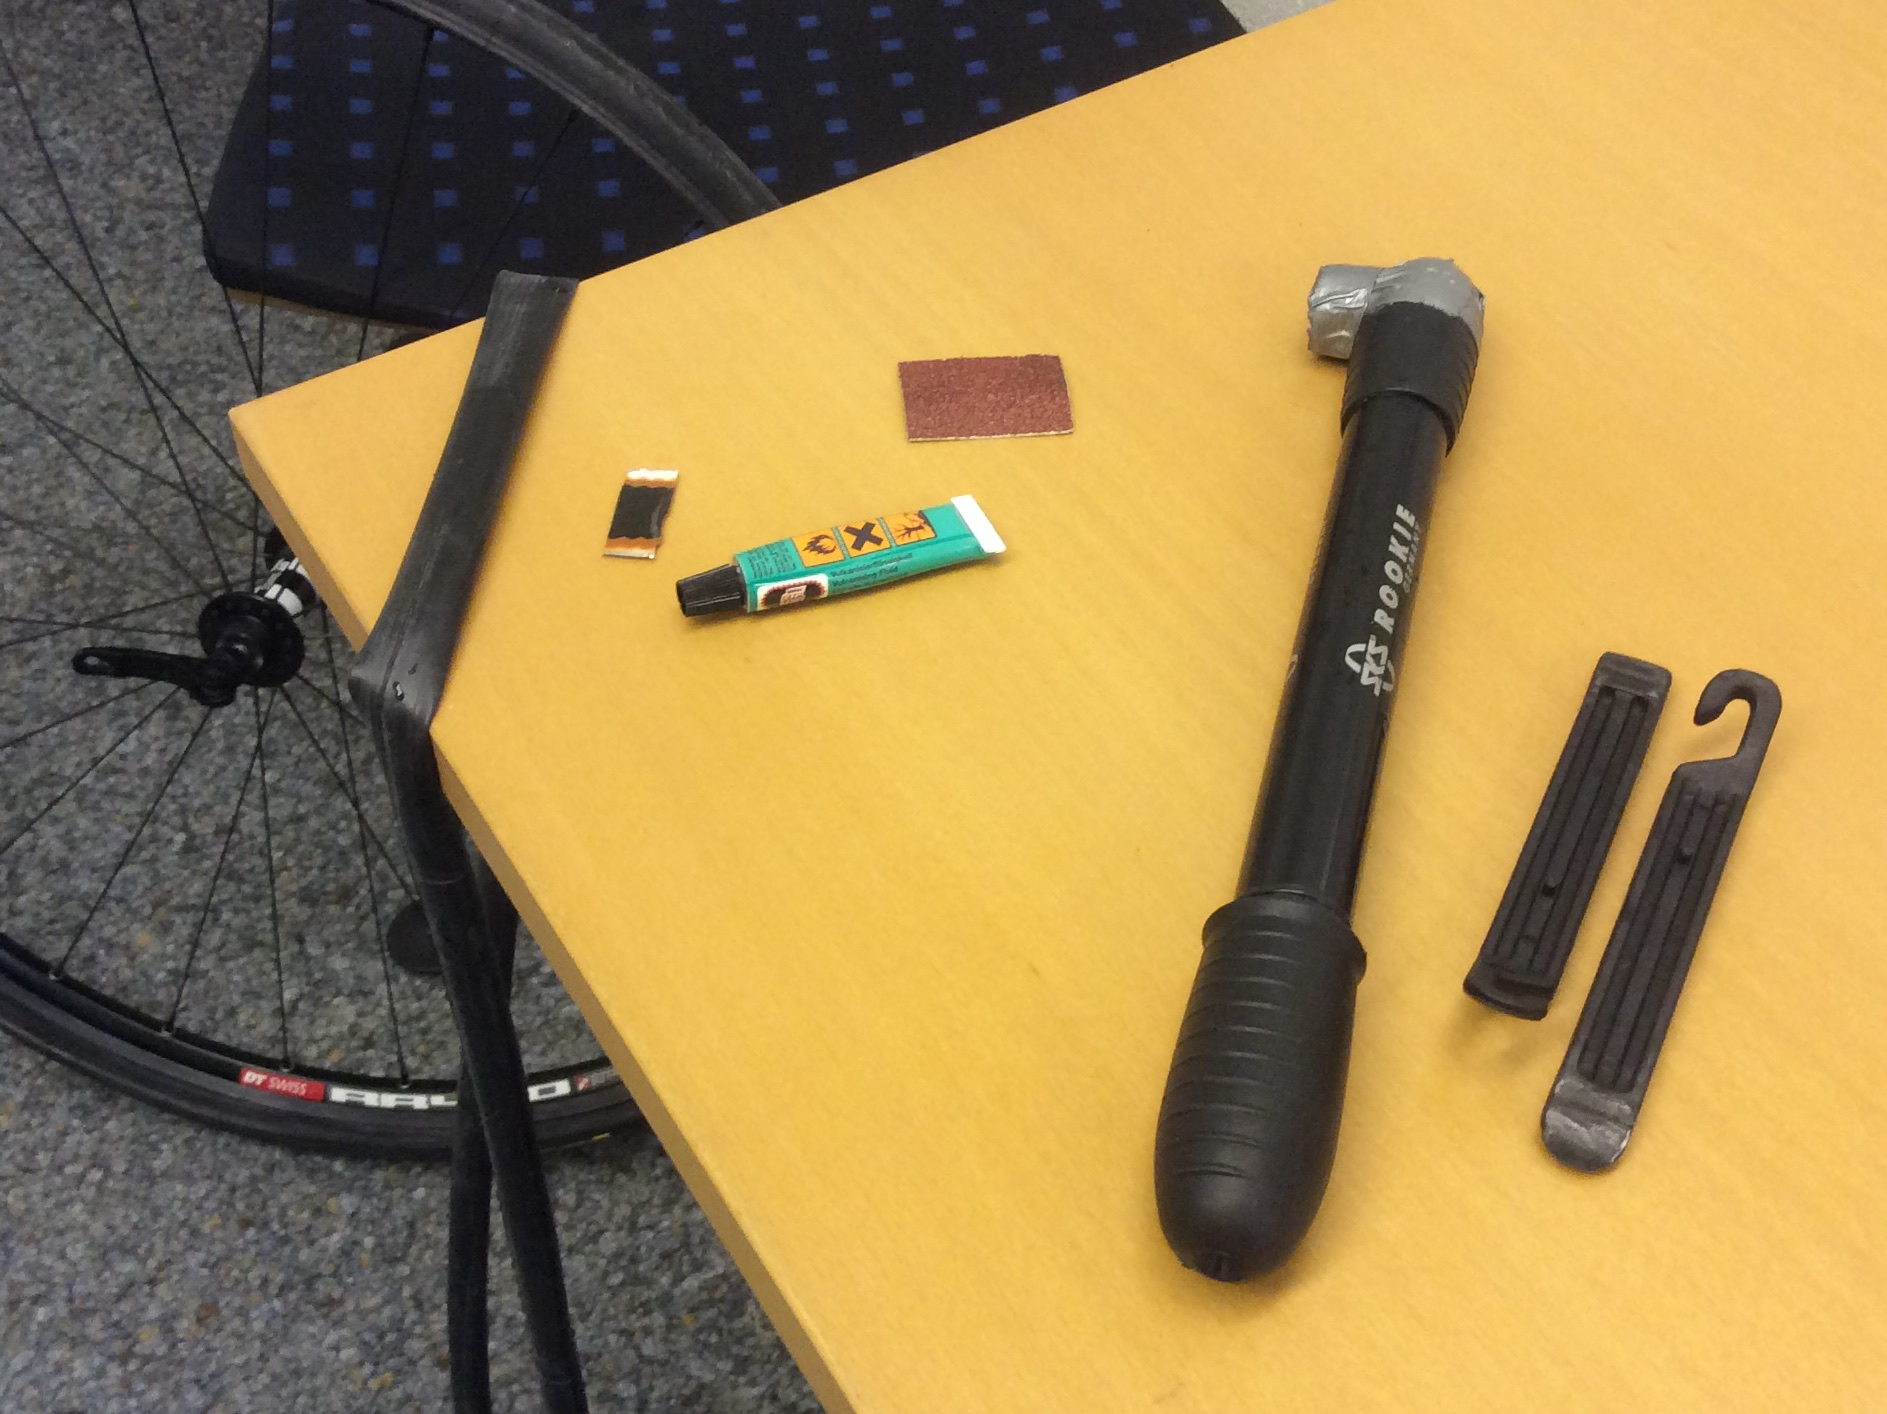
\includegraphics[width=\textwidth]{figures/reparatur-arbeitsplatz.jpg}
        \caption{Reparatur am Arbeitsplatz}
        \label{fig:reparatur-arbeitsplatz}
\end{figure}


\section{Wieso ein Rennrad zum Pendeln}

Es gibt durchaus Gründe, wieso man eher ein Trekking- oder Fitness-Bike als ideales Pendler-Rad sehen kann \cite{Lindthaler2015perfektesfahrradpendler}.



Möglichkeit der Reparatur unterwegs oder am Zielort (Arbeitsplatz, zu Hause). Möglichkeit einer Alternative (ÖV, Taxi).
Reparatur am Arbeitsort
Gelegentlich passiert einem etwas auf dem Weg zur Arbeit. Wenn man das Rennvelo dann reparieren kann, erspart man sich viel umtriebe (Transport des nicht mehr fahrtauglcihen Rades nach Hause, dortige Reparatur). Kleine Reparaturen wie platter Reifen usw. macht man am besten in einer Arbeitsplause oder über Mittag.
Regeneration, Wiederherstellen des Betriebszustand

Das Rennrad muss regelmässig gewartet werden.

Kleine Reperaturen deshalb gleich am Abend machen, am Wochenenden oder freien Tagen einen umfassenden Check (Bremsen, Kette) und Unterhaltsarbeiten.
Je länger man mit Wartungsarbeiten zuwartet, desto umfagreicher werden erfahrungsgemäss die Reparaturen.
Auch eine wichtige Erfahrung: wenn einem beim Fahren etwas auffällt (Geräusch, komisches Gefühl), dann sollte man unbedingt dem nachgehen.
Ignorieren oder Verdrängen (<<Da wird schon nichts sein>>) bringt \emph{todsicher} Probleme.
Irgendwann ist dann die lockere Schraube ganz weg und eine Reparatur, die bei besserer Aufmerksamkeit ein paar Sekunden gedauert hätte,
wird ein Steckenbleiben am blödsten Ort und eine umfangreiche und teure Reparatur.


\section{Bekleidung}

Der Fokus ist hier eher bei Outdoor-Bekleidung als bei \emph{richtiger}, d.h. wettkampforienierter Rennradbekleidung.

Schuhe mit weicher Sole

Übershuhe als Regenschutz.

\section{Restliches Material}




\chapter{Organisation}

\section{Vorbereitung ist alles}

Vorbereitung ist der Schlüssel für Effizienz.
Die Vorbereitung für ein Pendeln mit dem Rennvelo

Ein Tagesablauf mit optimaler Verbindung von Pendeln, Training und Arbeit.

\subsection{Vorabend}


\section{Wie lange ist die Fahrzeit?}

Die Fahrzeit berechnet sich $t = s/v$.
Für einen Arbeitsweg von 10\,km und einer Durchschnittsgeschwindigkeit von 30\,km/h kommt man also auf $10/30=0.33$.
Multipliziert mit 60 ergibt die Zeit in Minuten, hier also 20\,min, siehe Tabelle \ref{tab:fahrzeit}.

Die Durchschnittsgeschwindigkeit auf dem Rennvelo ist stark abhängig von der Strecke (flach vs. hüglig) und von den Windverhältnissen.
Kräftiger Gegenwind kann die Durchschnittsgeschwindigkeit um 5\,km/h drücken.
Hier hilft die vorgängie Konsultation des Wetterberichtes.
Muss man aufgrund der Witterungsverhältnissen einmal auf's MTB umsteigen, dann ist man ebenfalls 5 -- 10\,km/h langsamer.
Die Tabelle \ref{tab:fahrzeit} hilft, sich dabei zu orientieren.
So kann abgeschätzt werden, wieviel länger man für den Arbeitsweg braucht,
sollten einem einmal die Witterung auf das MTB zwingen.

\begin{table}
        \centering
        \begin{tabular}{cccccc}
                \toprule
            &	10\,km	&   20\,km	& 30\,km	&   40\,km	& 50\,km    \\
    \midrule
20\,km/h	&   30      &	60	    & 90        &   120	    & 150       \\
25\,km/h	&   24      &	48 &	72 &	96 &	120  \\
30\,km/h	&   20      &	40 & 	60& 	80 &	100 \\
35\,km/h	&   17      &	34 &	51& 	69 &	86 \\
40\,km/h	&   15      &	30 &	45& 	60 &	75 \\
\bottomrule
        \end{tabular}
        \caption{Fahrzeit in Minuten, abhängig von der Distanz und der Durchschnittsgeschwindigkeit.
        (MTB minus 5 -- 10\,km/h, Gegenwind minus 5\,km/h).
        Anwendung:
        wird die Strecke zur Arbeit 20\,km mit den Rennvelo bei einer Durchschnittgeschwindigkeit von
        30\,km/h gefahren,
        dann wird man mit dem MTB wohl 8 Minuten (48 - 40) länger haben.}
        \label{tab:fahrzeit}
\end{table}

\section{Transportierendes Material}

\begin{table}
  \centering
  \begin{tabular}{ll}
    \toprule
        Was?    & Kommentar \\
    \midrule
        Schlüssel, Handy, Geldbörse     & Essentials \\
        Notfallwerzeug für Panne        & Siehe näheres unter entsprechendem Abschnitt \\
        Regenschutz, Überschuhe         & Fahrradbezogene Dinge \\
        Wäsche, frisches Hemd           & jeden Tag, nach dem Duschen \\ 
        Verpflegung Tag                 & Entfällt bei Kantinenverpflegung \\
        Geschäftsunterlagen             & Berufsbezogene Unterlagen \\
    \bottomrule
  \end{tabular}
  \caption{Eine Aufstellung der Dinge, die täglich transportiert werden müssen.}
  \label{tab:transportmaterial}
\end{table}



\section{Hygiene}

Ich mache am Arbeitsplatz eine kleine Sport- oder Strandtasche mit allem nötigen parat (Abb. \ref{fig:sporttasche}).
Glücklich, wer eine eigentliche Garderobe mit abschliessbarem Schrank hat.

Aufhängen der Wäsche im Büro.
Um nasse oder verschwitzte Klamotten kommt man nicht herum.
Schön ist, wenn man diese im Büro aufhängen kann.
Allerdings sollte man die Aversion, die solche Klamotten oder nassen Handtücher auslösen können, nicht unterschätzen.
Was für einem selber die ultimative Trophäe und Beweis seiner Leistungsfähigkeit ist, ist für andere nur eine blanke Zumutung.

\begin{figure}[htpb]
        \centering
        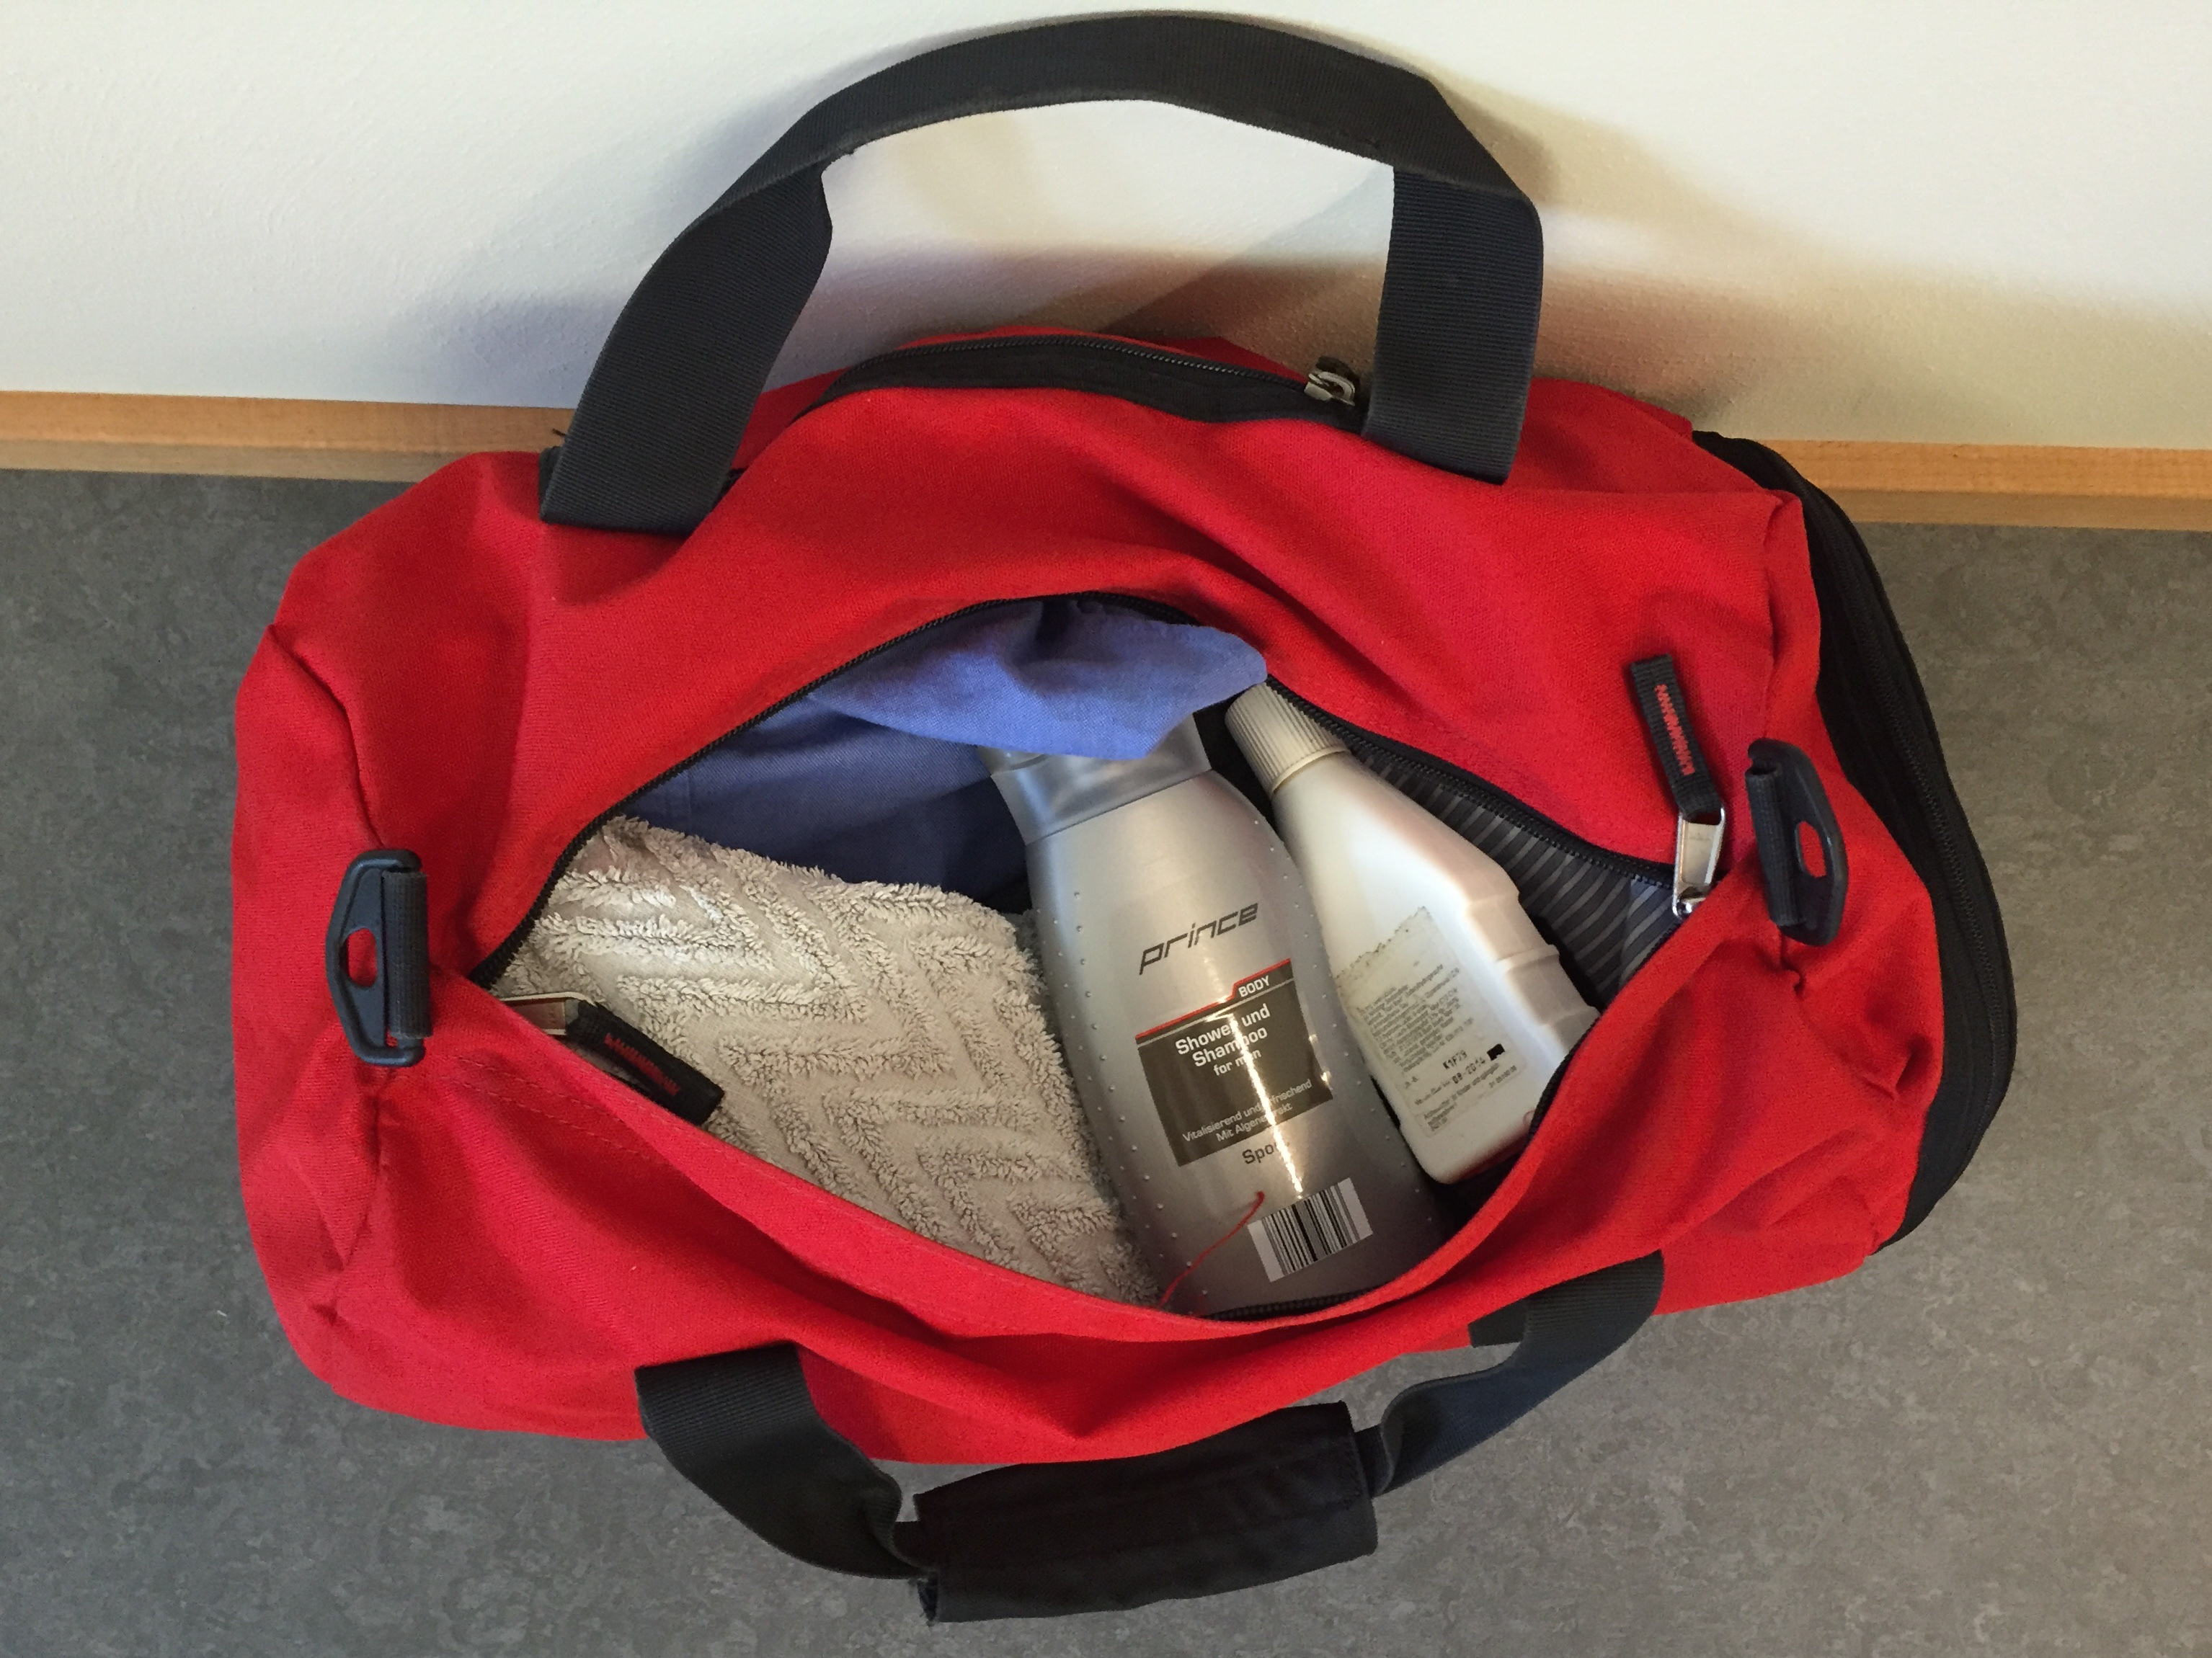
\includegraphics[width=\textwidth]{figures/sporttasche-gepackt.jpg}
        \caption{Im Büro ist eine immer gepackte Sporttasche, in der die Wechselkleider und das Duschzeugs ist.}
        \label{fig:sporttasche}
\end{figure}

\chapter{Pendeln und Training}

\shorthandoff{"}
    \dictum[\citeNP{sollritchey2011rennradnews}]{
        "Ich fahre jeden Tag 33 km einfach zur Arbeit und das bei JEDEM Wetter.
        [\ldots]. Im Winter gibt es kein besseres Training,
        ohne Arbeit würde ich diese km Leistung niemals fahren"
        }
\shorthandon{"}

\section{Problematik}

Bei 100prozentigem Arbeitspensum und allenfalls Familie noch genügend Zeit
für ein seriöses Rennrad-Training aufzubringen ist eine Herausforderung.
Eine mögliche Lösung ist das regelmässige Pendeln mit dem Rennrad (road
bike commuting). In diesem Artikel werden die Schwierigkeiten und mögliche
Lösungen zum Pendeln mit Rennrad (PmRR) dargestellt. Der Autor kann dabei
auf mehrere Jahre Erfahrung mit einem Wochenschnitt von ca. 100 km pendelnd
zurückschauen.

Pendeln zum Arbeitsplatz und Rennrad-Training sind zwei unterschiedliche
Tätigkeiten, die sich nur in einem kleinen Bereich überschneiden, nämlich
in der Eigenschaft, dass man sich (möglichst schnell) vom Punkt A nach Punkt
B bewegt.

In vielen anderen Bereichen sind hier konträre Ziele: beim Pendeln will man
möglichst grosse Flexibilität, gepaart mit möglichst viel Bequemlichkeit.
Man muss oft Dinge (Unterlagen, Bücher, Equipment) transportieren. Der
Arbetisplatz stellt Anforderung an Erscheinungsbild (Hygiene, Kleidung). Der
Arbeitsplatz muss pünktlich erreicht werden -- dies auch bei schlechtem
Wetter oder bei Dunkelheit. Auch will man pünktlich wieder zu Hause sein.

Beim Rennrad-Training will man möglichst \emph{wenig} mitnehmen auf einem
Rad, dass möglichst leicht ist. Die Kleidung soll für das Rannradfahren sehr
funktional sein. Um den Trainingeffekt zu optimieren ist es unvermeidlich,
dass man Schwitzt. Rennradfahren bei Dunkelheit, viel Verkehr oder schlechten
Wetter wird -- wenn möglich -- vermieden.

Vorteile:
\begin{itemize}
        \item Zeit, die man für den Arbeitsweg aufbringt wird als Trainingszeit genützt.
        \item Das Training wird am Tag gesplittet.
        \item Allenfalls Kostenersparnis gegenüber der Benutzung von anderen privaten Verkehrsmitteln (Auto) oder öffentlichem Verkehr.
        \item Keine Abhängigkeit von öffentlichem Verkehr.
\end{itemize}
\section{Faktoren des Trainings}

Häufigkeit, Dauer, Intensität

\section{Häufigkeit}

\section{Dauer}

\begin{table}
        \centering
        \begin{tabular}{ccccccccccc}
                \toprule
&	5	& 10	& 15	& 20	& 25	& 30 & 35	& 40	& 45	& 50\\
    \midrule
1 &	480	& 960	& 1440	& 1920	& 2400	& 2880	& 3360	& 3840	& 4320	& 4800 \\
2 &	960 &	1920 &	2880 &	3840 &	4800 &	5760 &	6720 &	7680 &	8640 &	9600 \\
3 &	1440 & 	2880 &	4320 &	5760 &	7200 &	8640 &	10080 &	11520 &	12960 &	14400 \\
4 &	1920 &	3840 &	5760 &	7680 &	9600 &	11520 &	13440 &	15360 &	17280 &	19200 \\
5 &	2400& 	4800 &	7200 &	9600 &	12000 &	14400 &	16800 &	19200 &	21600 &	24000 \\
\bottomrule
        \end{tabular}
        \caption{Jahreskilometer abhängig von der Strecke Wohnort-Arbeitsort sowie der Anzahl Tage, an denen mit dem Rad gependelt wird.}
        \label{tab:jahreskilometer}
\end{table}

\section{Intensität}




\chapter{Sicherheit}

\section{Diebstahlschutz}

Etwas vom Allerärgerlichsten ist wohl der Diebstahl des Rades. Geschichen,
von Personen, die sich <<nur kurz umgedreht haben>>, und das neue, teure
Carbon-Rad war weg gibt es genug. Die Situation wird für Pendler, die das
Rad an einem öffentlichen Ort oder auf dem Firmen-Rad-Unterstand für die
Arbeitszeit anbringen müssen, nicht wirklich besser

\begin{enumerate}
  \item Das Rad immer an einem festen Gegenstand sichern. Das Abschliessen von Vorder- oder Hinterrad ist bloss eine 
    Wegfahr, aber keine Wegtragsperre.

  \item Beim Abschliessen darauf achten, dass das Verschlusssystem (Kette, Bügelschloss) eng sitzt.
    Dies um einem Dieb möglichst wenig Arbeitsraum zu bieten. Das Schloss soll möglichst nach unten zeigen und
    schwer zugänglich sein.

  \item Das Rad für den Arbeitsweg sollte eher vom Typ <<Stadtschlampe>>, als dem ultimativen Renner sein.
    Siehe dazu auch das Kapitel <<Welches Rad?>>

  \item Mit zwei Rädern und zwei Schlössern kann man Schliessgemeinschaften bilden.
    Ein Dieb muss so zwei Schlösser knacken, um sich mit der Beute aus dem Staub machen zu können.

  \item Entgegen dem Impus, das Rad etwas <<verstecken>> zu wollen, wähle eine belebte Stelle um das Rad zu sichern.
    Auf grossen Rad-Abstellplätzen eine vordere Reihe wählen.
    Im Blick der Passanten ist das Rad besser geschützt.
    Mir ist es allerdings schon passiert, dass ich das eigene Rad wg. eines Schlossdefektes selber knacken musste.
    Obwohl ich dabei mit einem grossen Bolzenschneider in aller Öffentlichkeit vorging, wurde ich nicht aufgehalten.
    Der oft geäusserte Tipp scheint also nur sehr beschränkt zu wirken.

  \item Ersatz von Schnellspannern an Laufrad oder Sattel mit herkömmlicher Schraube ersetzen.
    Es gibt auch sog. Tamper-proofe Schrauben -- für den Sattel. Allerdings muss man dann auch die entsprechenden WErkzeuge
    für eine Panne mitführen. Allenfalls hat dann bei einer Panne auch ein Bike-Werkstatt das entsprechende Werkeug nicht.

  \item Was sind die sichersten Rad-Schlösser? Mögliche Kaufempfehlung bietet http://www.trelock.de/

\end{enumerate}

\section{Einhalten von Verkehrsregeln}
Ein wichtiger Punkt zur Risikosenkung scheint mir das Einhalten der Verkehrsregeln. Der Arbeitsweg ist i.d.R. nicht ein idealer Velo-Weg. Oft ist der Verkehr nicht entflochten und das Verkehrsaufkommen ist gross. Zudem sind Autopendler oft gestresst, abgelenkt, müde.  Das peinliche Einhalten von Verkehrsregeln scheint mir aus folgenden Gründen angepasst:
Das Risiko wird erheblich gemindert. Man wird für die anderen Verkehrsteilnehmer berechenbarer.
Man provoziert keine anderen Verkehrsteilnehmer.
Sollte tatsächlich etwas passieren, ist man rechtlich auf der sicheren Seite.
\cite{Flieshardt2015}

\subsection{Strassenverkehrsregeln Radfahrer Deutschland}
\citeNP{Flieshardt2015}
\begin{itemize}
        \item Radwegbenutzung: Bezeichnete Radwege (Zeichen 237, 240, 241) müssen benutzt werden. Ansonsten ist die Nutzung von Radwegen freiwillig.
        \item Nebeneinanderfahren: Solange der Verkehr nicht behindert wird. 
        \item Einbahnstrasse in Gegenrichtung: Erlaubt mit Zusatzschild <<Radfahrer frei>>.
        \item Musik hören: Warnsignale müssen wahrgenommen werden.
        \item Beleuchtung: Front- und Rücklicht müssen jederzeit mitgeführt werden. Akkulampen benötigen ein StVZO-Siegel.
\end{itemize}

\subsection{Strassenverkehrsregeln Radfahrer Oesterreich}
\begin{itemize}
        \item Radwegbenutzung: Radwege müssen benutzt werden. Trainierede Rennradfahrer sind von der Pflicht ausgenommen.
        \item Nebeneinanderfahren: im Training erlaubt. 
        \item Einbahnstrasse in Gegenrichtung: Gestattet, wenn Erlaubnis gesondert beschildert.
        \item Musik hören: nicht geregelt, kein ausdrückliches Verbot
        \item Beleuchtung: müssen bei guter Sicht nicht mitgeführt werden.
\end{itemize}

\subsection{Strassenverkehrsregeln Radfahrer Schweiz}
\begin{itemize}
        \item Radwegbenutzung: müssen auch von Rennradfahrern benutzt werden
        \item Nebeneinanderfahren: bei geringem Verkehr erlaubt.
        \item Einbahnstrasse in Gegenrichtung: Erlaubt wenn gesondert ausgeschildert.
        \item Musik hören: Erlaubt, wenn Warnsignale wahrnehmbar sind.
        \item Beleuchtung: müssen bei guter Sicht nicht mitgeführt werden.
\end{itemize}

\section{Helm}

\section{Licht/Reflektoren}

Genügend Licht ist unverzichtbar. Es gibt nur wenige Sommermonate, wo man mit Sicherheit bei vollem Tageslicht zur und von der Arbeit kommt.
Meist wird es schon im September morgens schon so dunkel, dass es die Sicherheit gebietet, sich mit Licht zu behängen.

Optimalerweise nimmt man eine Lampe am Lenker und am Helm. Licht am Helm hat den vorteil, dass man bei einer Kopfbewegung
noch weitere Teile ausleuchten kann (Kettenposition!). Man wird aber auch wg. der erhöhten Pos. des Lichtes
von Verkehrsteilnehmer besser wahrgenommen.


\chapter{Arbeitplatzaspekte}

\section{Positive Aspekte für die Arbeit}

\section{Negative Aspekte}

\subsection{Nicht mit sportlichen Erfolgen angeben}

Wer wöchentlich 100\,km oder mehr auf dem Rad zurücklegt ist in Kreisen von Fitness-Websites wie Strava und Fitocracy allenfalls Durchschnitt.
Hier ist Raum um sich mit den sportlichen Leistungen zu brüsten.
Vorsicht ist allerdings Geboten herausposaunen der sportlichen Leistungen vor Arbeitskollegen, insbesondere auch Untergebenen und Vorgesetzten.
Es kann sein, dass hier auch Neid mitspielt, aber wer zu sehr auf seine sportlichen Erfolge pocht,
der stösst in durchschnittlich sportlichen Kreisen der Couch-Potatos durchaus auf Ablehnung.
Inbesondere wenn Absenzen durch Krankheit, Unfall oder Wettkämpfe dazukommen.
Die berufliche Leistung darf auf gar keinen Fall darunter leiden, sonst kann man sicher sein, dass man schnell als "Verrückter" oder "Narzisst" gilt.

Ohne Optimierung der Abläufe lässt sich ein Vollzeitjob und intensives Training nicht verbinden \cite{Roemer2014ironmanvollzeitjob}.
In diesem Artikel von Römer wird auch Michael Krell zitiert: <<Hobbysportler [sollten] im Beruf eher sparsam mit Geschichten zu ihrem Trainingseifer umgehen>>,
<<Auf keinen Fall darf bei Chefs der Eindruck entstehen, dass der Sport die Arbeit negativ beeinflusst ...>>.

Etwas \emph{low profile} kann also nicht schaden.

\subsection{Vorsicht mit sozialen Medien und Surfen}

Ich würde insbesondere hier auch auf eine strikte Trennung von Privat und Geschäft raten.
Stöbern in Rennrad-Foren, Unterhalten eines (Sport-)-Blotg, Nachfüren von Webeinträgen in Strava und Fitocracy sind meines Erachtens totale No-Gos am Arbeitsplatz.



\chapter{Schlechtes Wetter}

\shorthandoff{"}
\dictum[\citeNP{nordwind2012rennradnews}]{"Direkt nach den Aufstehen aus dem Fenster geguckt und es war am Regnen und sehr Windig,
20min später losgefahren und siehe da der Regen hatte auf gehört und ich hatte den kompleten Weg zur Arbeit Rückenwind wie doof."}
\shorthandon{"}

\section{Kognitive Umstrukturierung}

Wenn man sich entscheidet, mit dem Rennrad zu pendeln
gehört eine positive Grundhaltung zu \emph{jedem} Wetter dazu.
Es ist durchaus so, dass ich bei mildem, sonnigen Wetter
(nicht zu heiss, nicht zu kalt) am liebsten fahre.
Nun ist das halt oft nicht der Fall.
Die Schweiz hat gleichmässig etwa 12 bis 14 Regentage pro Monat.
D.h. dass im Schnitt es so an jedem dritten Tag mit Regen zu rechnen ist.
Wenn man Glück hat, sitzt man nicht gerade im Sattel,
wenn dieses Nass vom Himmel kommt, sondern vorher oder nachher.
Trotzdem ist mit Nasswerden auch bei optimaler Planung und Studium
des Wetterbrichtes immer zu rechnen.

Ein weiterer Trick ist, sich selbst kognitiv neu zu strukturieren
(sprich: die Sache positiv zu sehen).
Zum Beispiel sich bewusst zu machen, dass die relativ kurze Distanz zur Arbeit nicht ausreicht, 
um wirklich auszukühlen oder wie Bradley Wiggins meint:
<<It's not really long enough to get super-cold>> \cite{bbc2015wigginswinter}.

Eine schöne Liste von Sportausreden und ihre Lösung hat Christiane Scholz (alias Anna Achilles)
zusammengetragen \cite{Scholz2016Sportausreden}.
Die schönste ist, <<Die Witterung als Gegner sehen. Schönwetter kann jeder.
Aber je kälter und ekliger es draußen ist, umso besser.
Ich mag den sportlichen Wettkampf. Das Duell. Statt Frau gegen Frau,
Frau gegen Wetter. Wann sonst hat man beim Laufen schon mal einen direkten Rivalen?
Wettergott! Schneewehen und eiskalter Ostwind - ist das alles, was du hast?!>>

Eine Routine hilft gegen den kläffenden, inneren Schweinehund.
Wenn alles für den morgen bereitliegt dann ist der Aufwand such umzuentscheiden viel größer.
Die Radklamotten liegen säuberlich bereit, die Straßen Klamotten sind <<versteckt>>.
Dabei ist A der Aufwand für Start mit Rennvelo und B der Aufwand für Start mit Auto/Zug.
Wenn A größer als B ist, ist die Chance gross, dass man sich aufs Rad schwingt.

Ein weiterer, wichtiger, gedanklicher Punkt ist der Umstand, dass nicht jedes Regenwolken-Symbol
auf dem Smartphone gleich bedeuted, dass man nass wird \cite{srf2016regenpoker}.
Man soll bei einer Regenprognose auf die Regenwahrscheinlichkeit und die Regenmenge schauen.
Sind beide tief, ist Regen kaum ein Thema. Aber auch einer hohen Regenwahrscheinlichkeit und
tiefer Regenmenge (oder umgekehrt) ist die Wahrscheinlichkeit hoch, dass man trocken bleibt.
Aber noch besser ist doch, wenn man sich kleidertechnisch und mental so vorbereitet,
dass allfälliger Regen kein Thema ist.

Für weitere Beispiele für die persönliche kognitive Umstrukturierung
siehe Tabelle \ref{tab:kognitiveumstrukturierung}).

\begin{table}
        \centering
        \begin{tabular}{l}
                \toprule
        <<Nach 5 Minuten im Sattel spüre ich das Wetter nicht mehr.>>\\
        <<Genau jetzt hole ich mir den Trainingsvorteil gegenüber Schönwetterfahrern.>>\\
        <<Jetzt verbessere ich meine Fahrtechnik in Nässe und Kälte.>>\\
        <<Ich hole mir jetzt Rennhärte!>>\\
        <<Bei schönem Wetter fahren kann jeder.>>\\
        <<Nichts ist schöner, als nach einer solchen Fahrt unter die warme Dusche zu stehen.>>\\
        <<Ich konzentriere mich auf die Strecke/den Belag/die Kadenz, dann spüre ich den Regen nicht mehr.>>\\
        <<If you are out riding in bad weather, it means you are a badass. Period. \cite[Rule \#9]{velominati2014rules}\\
                \bottomrule
        \end{tabular}
        \caption{Kognitive Umstrukturierung: wichtig ist dabei sich einen für sich stimmige Grundüberzeugung zu finden.
        Diese muss dann möglichst oft ins Bewusstsein geholt werden, um verankert zu werden.}
        \label{tab:kognitiveumstrukturierung}
\end{table}

\section{Fahren bei Kälte}

\textbf{Luftdruck der Reifen reduzieren:}
Erhöht den Gripp des Reifens. 

\textbf{Vorsicht bei heiklen Stellen:}
Strecken im Schatten, am frühen Morgen oder über Brücken bergen bei Kälte Glatteisrisiken.

\section{Fahren bei Regen}
\label{sec:regen}

Regen heisst in unseren Breitengraden: es ist Kalt \emph{und} Nass.
Das Thema Kälte wurde soeben angeschaut, hier kommt noch der Teil mit dem Nass.

Folgende Hinweise von
\cite{Glass2014cyclingrain,Hurford2014rainyride,Prinz2014rain,Lovell2015tipswetweather,gcn2013rain,gcn2015rain}

Zur Motivation bei Fahrt im Regen \cite{Magnuson2013rain}

\subsection{Massnahmen am Rad}

\textbf{Schutzbleche montieren:}
<<Schutzbleche sind unästhetisch und gehören nicht ans Rennvelo.>>
Die, die so denken, fahren nicht oft bei Regen.
Nichts kann einem die Freude am Fahren schneller vermiesen als von unten mit dem ganzen Strassenschmutz bespritzt zu werden.
Zudem irrigiert der dauernd benässte Hintern. Ein nicht zu vernachlässigendes Sicherheitsrisiko.
An das Pendler-Rad gehören Schutzbleche.
Gepfiffen auf die Ästhetik -- oft ist ja sowieso dunkel.
Es geht ja auch um dem Trainingseffekt -- da stören die wenigen Gramm, die entsprechende Schutzbleche wiegen kaum.

\textbf{Breitere Reifen montieren:} 
Insbesondere bei Scheibenbremsen besteht die Möglichkeit, breitere Reifen zu montieren.
Das erhöht die Kontaktfläche Gummi--Strasse.

\textbf{Licht montieren:}
Ich spreche hier nicht von den kleinen Designerlämpchen, die man im Fahrradzubehör für die Rennradfraktion bekommt.
Ich spreche von \textbf{Licht}!
Ich spreche Super-Mega-Watt-Funzeln, die durchaus geeignet sind,
mit ihrem Lichtkegel fortlaufend die Strasse vor einem zu trocknen.
Erhältlich nur gegen Waffenschein im MTB-Zubehör.
Alles anderes ist Etepetete-Klinkerlitzen-Spielzeugkram.

\begin{figure}[htpb]
  \centering
  
\includegraphics[width=0.5\textwidth]{figures/ohne-beleuchtung.jpg}
  \caption{Aus einem Facebook-Post \protect\cite{officepony2016organspendeausweis}},
  \label{fig:ohne-beleuchtung}
\end{figure}

\textbf{Kettenöl}
Nicht jedes Kettenschmiermittel ist für Nässe gleich geeignet. So sind die Trockenschmiermittel
für Nassfahrten weniger geeignet als Kettenöl.

\subsection{Kleidung/Ausrüstung}

\textbf{Brille:}
Ob jemand eine Brille bei Regen trägt, hängt meines Erachtens von der Situation ab.
Je nach Licht, Verkehr, Regenstärke finde ich eine Brille hilfreich oder störend.
Oft fahre ich dann ohne Brille.
Allerdings benutze ich Schutzbleche.
Ohne, dient eine Brille auch als Schutz von Spritzer von Regen und hochgeschleudertem Strasendreck dienen sie auch der Sicherheit.
Ausgerüstet mit gelben oder orangen Gläsern, erhöhen sie den Kontrast.

\textbf{Radfahrerkappe unter Helm:}
Neben dem Profi-mässigen Aussehen dient der Schirm noch etwas dazu, die Augen zu schützen.
Allenfalls entschliesst man sich sogar für den Kauf eines MTB-Helmes mit Schirm.

\textbf{Überzieh-Handschuhe:}
Als meine Wetter-Schwachstelle würde ich die Finger bezeichnen.
So ungerne ich an die Finger friere, so ungern habe ich es dort zu warm.
Diesbezüglich habe ich ein kleines Sortiment an unterschiedlich gefütterten Handschuhen.
Neben den wasserfesten Winterhandschuhe (gegen Nässe und Kälte) gibt es im Handel auch dünne Sommer-Regen-Überziehhandschuhe
(z.B. Roeckl Malvas).
Wem auch eine unkonventionellen Lösung genehm ist und damit leben kann, auf dem Rennvelo wie ein Chirurg auszusehen,
kann sich im Falle eines Wolkenbruches auch ein Paar Latex-Handschuhe überziehen.
Ich persönlich werde dann halt lieber nass.

\textbf{Regenüberschuhe/wasserdichte Socken:}
Die Regenüberschuhe sollten so beschaffen sein, dass sie einfach an- und ausgezogen werden.
Ich führe \emph{immer} ein Paar im Rucksack.
Wenn die Radschuhe erst einmal so richtig durchnässt sind,
kann es Tage gehen, bis sie wieder trocken sind.

\textbf{Regentaugliche Kleidung:}
Grundsätzlich sollte gerade bei Regen auf leuchtende, reflektierende Kleidung getragen werden.
Je bunter desto besser?
Mit der üblichen Funktionskleidung wirkt man bei der Normalbevölkerung sowieso etwas seltsam \cite{Rasche2016albern}.
Aber eigentlich ist egal, was andere denken, wenn es der eigenen Sicherheit und Komfort dient.
Bei Nässe kann man sich für grundsätzlich für eine \textsl{hard shell} oder \textsl{soft shell} entscheiden.
Während eine hard shell mehr wasserdicht ist aber weniger Ventilation (Schweiss) zulässt
und eher für lange Ausfahrten geeignet ist \cite{gcn2015rain},
ist bei den eher kurzen, harten Fahrten zum Pendlen eine soft shell geeigent
(wohl weniger wasserdicht, lässt mehr ventilation zu, weniger Geflatter).
Gegebenenfalls muss man sich auch um Trocknungsgelegenheiten am Arbeitsplatz besorgt sein (Abb. \ref{fig:material-am-trocknen}).

\textbf{Rucksack mit Regenüberzug:}
Ist sicher tivial, scheint mir aber aus folgenden Punkten im Bezug aufs Pendeln erwähnenswert.
Mehr als früher montiere ich den Regenüberzug schon im Voraus.
Es nervt, bei der Fahrt wegen einsetzendem Regen anzuhalten und ihn nachträglich zu montieren.
Gerne lässt man es dann bleiben und ärgert sich dann über durchnässtes Arbeitsmaterial.
Zudem ist der Regenüberzug oft durch Farbgebung und Reflexionsstreifen noch etwas auffälliger als der Rucksack selbst,
was die Sicherheit erhöht.

\textbf{Handy in Gefrierbeutel:}
Wenn nicht schon im Rucksack lohnt sich für z.B. für das Handy ein Gefrierbeutel mit Clipverschluss.
Das mache ich auch bei trockenem Wetter zum Schutz vor Schweiss.

\textbf{Sitzcreme auftragen:}
Global Cycling Network empfielt noch speziell bei Regen das Auftragen von Sitzcreme \cite{gcn2013rain,gcn2015rain}.
Die Begründung des Schutzes der feuchten Haut leuchtet ein, das ist aber kaum nur ein Problem bei Regen,
die Stelle wird auch bei trockenen Ausfahrten nass durch den Schweiss.
Generall wird Sitzcreme (günstige Alternative ist Melkfett) bei langen Ausfahrten als Schutz vor dem Wundscheuern empfohlen.
Ob sich persönlich der Extraaufwand für die vergleichsweise kurze Strecke lohnt, muss jeder für sich ausprobieren.

\begin{figure}[htpb]
  \centering
  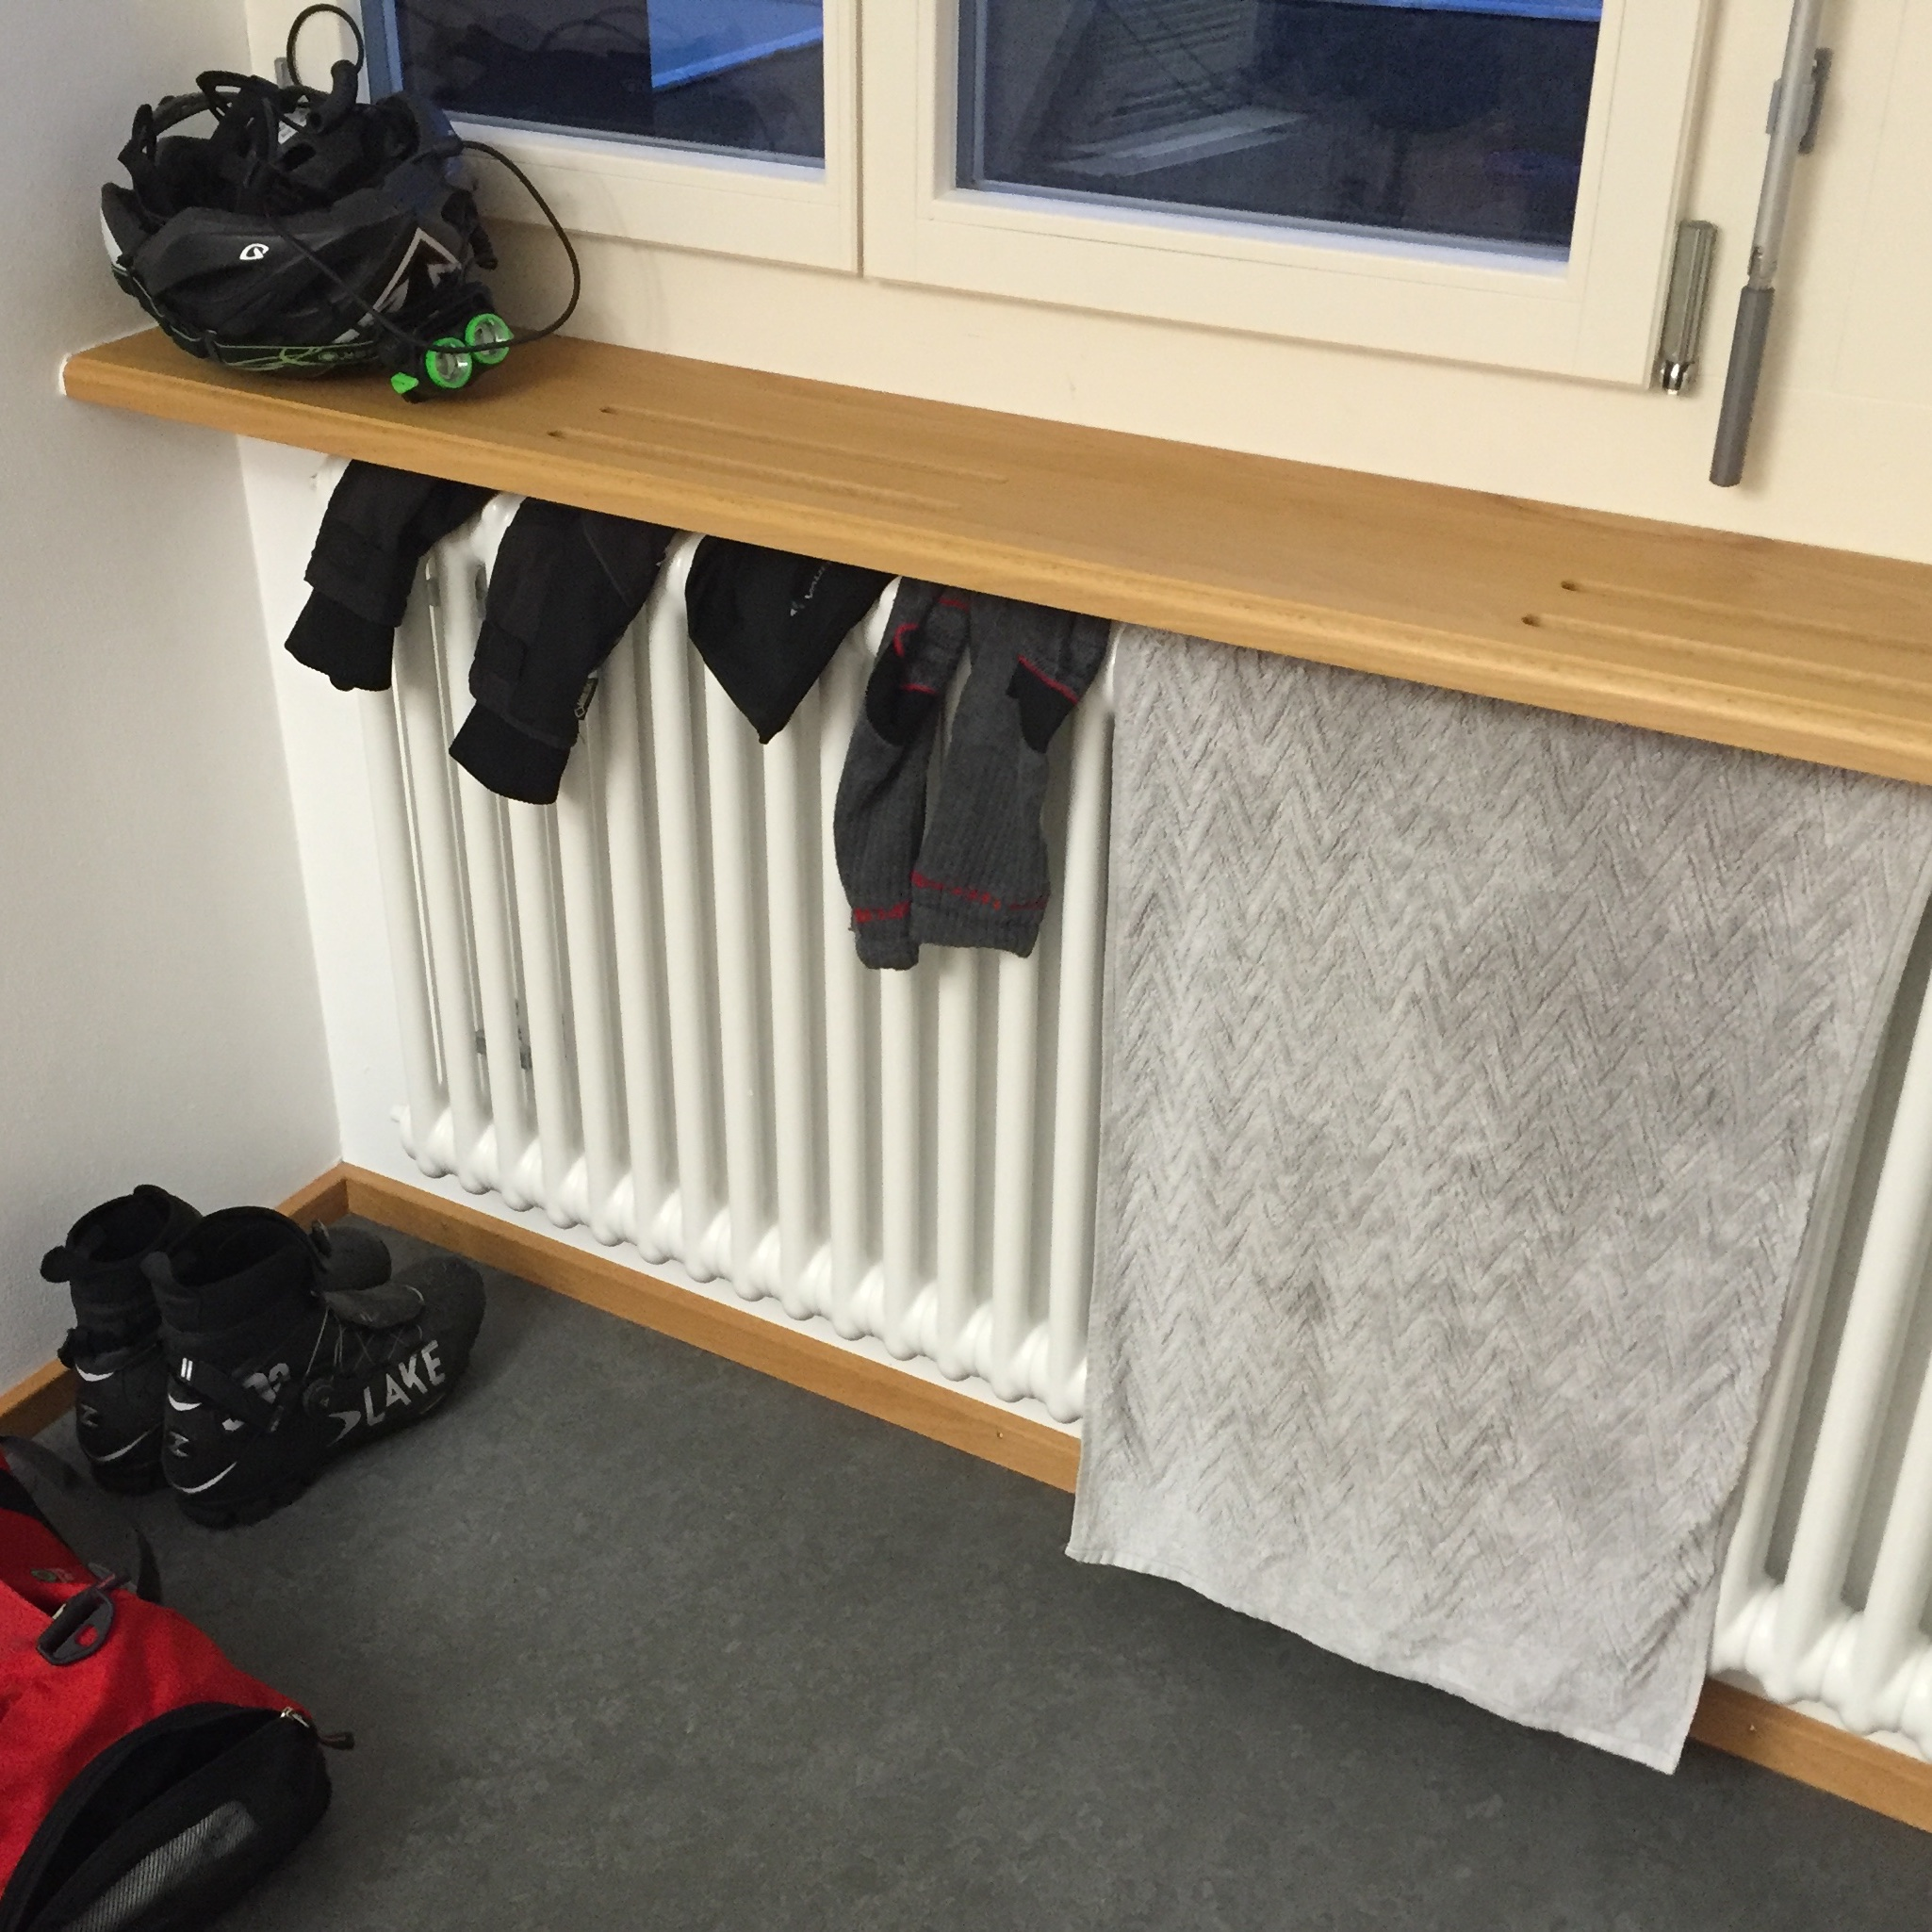
\includegraphics[width=0.8\textwidth]{figures/material-am-trocknen.jpg}
  \caption{Gehört auch zum Regen: Klamotten am Arbeitsort trocknen können.
    Vielleicht darf man Teile auch im Heizungsraum oder in der Gardarobe trocknen lassen?
    Den Hausmeister nett fragen schadet nicht.},
  \label{fig:material-am-trocknen}
\end{figure}

\subsection{Verhalten}

\textbf{Löcher und Pfützen meiden:}
Man soll dem kindlichen Impuls widerstehen, durch Pfützen zu fahren.
Auch unter einer harmlosen kleinen Wasserlache kann ein tieferes Loch oder eine Glasscherbe lauern.

\textbf{Vorsicht bei Strassensignalisationen, Gulli-Deckel, Tram-Schienen:}
Man soll sich das eigentlich schon bei trockenem Wetter angewöhnen.
Strassenbemalungen und Gullideckel sind tabu.
Insbesondere die Kombination Gummi und nasses Metall ist wie Schmierseife.

\textbf{Geschwindigkeit anpassen:}
Bei Nässe haften die Räder nur noch halb so gut wie im Trockenen (Tabelle \ref{tab:haftreibung}).
Neben der schlechteren Strassenhaftung ist die eigene Sicht stark eingeschränkt.
Zudem funktionieren die (Felgen-)Bremsen wie gewohnt.
Die Räder blockieren viel schneller, was den Bremseffekt weiter schwächt.

\begin{table}
  \centering
  \begin{tabular}{ll}
    \toprule
    Strassenzustand & Haftreibungungszahl \\
    \midrule
    trocken         & 0.7 -- 0.1 \\
    nass            & 0.4 -- 0.6 \\
    nasses Laub, Schnee & 0.2 -- 0.3 \\
    bei Eis         & 0.1 \\
    \bottomrule
  \end{tabular}
  \caption{Haftreibungszahl von Luftreifen bei verschiedenen Strassenzuständen \protect\cite{Strommer2016haftreibung}}
  \label{tab:haftreibung}
\end{table}


\textbf{Bremsen trocken bremsen:}
Gerade vor Kreuzungen oder geplanten Stopps kann man schon gefühlvoll etwas vorbremsen.
Man vermeidet so die Schrecksekunde, wenn die Felgenbremsen im Nassen nicht reagieren.

\textbf{Gefühlvoll in die Kurve:}
Weniger Haftung, schlechte Sicht.
Zwei Gründe, wieso gerade in der Kurve vorsichtig gefahren werden muss.

\textbf{Vorhersehbar fahren:}
Für andere Verkehrsteilnehmer mitdenken.
Gerade bei Regen ist die Sicht auch für andere Verkehrsteilnehmer eingeschränkt.
Umsomehr soll man alles vermeiden, was gerade Autofahrer irritiert (Slalom, Vortritt missachten).
Hypervorsicht und pingeliges Einhalten von Verkehrsregeln ist hier angesagt.

\textbf{Regenfahrt geniessen:}
Das scheint mir fast der wichtigste Punkt.
Keine Panik vor Regen!
Wenn man sich dem Wetter hingibt und in sich hineinfühlt merkt man plötzlich: es ist gar nicht schlimm.
Sondern es macht ja Spass!
Das Licht ist anderst, die Geräusche sind anderst. Man sieht die Tropfen vom Rad springen.
Man fährt anderst, weicht den Pfützen aus, vermeidet Gullis.
Regen auf dem Gesicht wäscht den Schweiss weg.
Man spührt, dass gegen die Hitze der Anstrengung die Kühle des Regens einem gut tut.


\chapter{Probleme des realen Lebens}

\section{Weitere Informationen}

Die Fahrstrecke kann genutzt werden, um Techniken (Haltung, Trittfrequenz, Wiegeschritt) zu üben.

Täglich an den gleichen Ort zu fahren, hat den Vorteil, dass man Feintuning betreiben kann.
Es empfiehlt sich, gefährliche Kreuzungen oder Strecken allenfalls zu umfahren oder eine Alternative zu suchen.
Auch kann mit der Abfahrtszeit gespielt werden. Schon 10 Minuten früher oder später kann bewirken, dass der Verkehr deutlich weniger ist oder weniger Lastwagen unterwegs sind.

Schlaglöcher sind mit der Zeit sehr vertraut und man kann schon frühzeitig eine andere Linie einschlagen.


\section{Fahrradtransport mit öffentlichen Verkehrsmitteln}

Die hier zusammengetragenen Informationen beziehen sich auf den Nahverkehr.
Oft sind abweichende Bestimmung im Bezug auf die Region oder des lokalen Verkehrsverbundes vorhanden.
Ein Problem ist auch, dass die einfache Fahrradmitnahme gerade zur Pendlerzeit oft nicht erlaubt oder
von (wenig planbarer) Einschätzung des Zugspersonal abhängig ist.
Insgesamt unproblematischer scheint es zu sein, das Fahrrad teildemontiert in eine entsprechende Tasche zu packen und als Handgepäck mitzuführen.

\subsection{Deutsche Bahn (http://www.bahn.de)}
Im Nahverkehr mit Fahrradsymbol kann das Fahrrad mitgenommen werden.
Zeiten mit Berufsverkehr sollen jedoch gemieden werden.
Eine ausdrückliches Mitnahmerecht besteht nicht und das letzte Wort hat das Zugspersonal. Zudem gibt es unterschiedliche Regelungen je nach Region.

Es gibt im DB Nahverkehr eine Fahrradtageskarte für \EUR{5}. Innerhalb von Verkehrsverbünden existieren teilweise abweichende Tarifbestimungen.

Als Handgepäck: Auf der Website der Bahn finden sich keine ausdrücklichen Angaben zur Mitnahme des verpackten, teilzerlegten Fahrrades.
Erfahrungsberichte bestätigen aber die Möglichkeit der Mitnahme.

\subsection{Österreichische Bundesbahn (http://www.oebb.at)}
Im Nahverkehr kann die Fahrradmitnahme nur bei genügend freien Stellplätzen erfolgen.
Ein Fahrradticket kostet 10\% des Vollpreises der 2. Klasse, mindestens aber \EUR{2}.
Es gibt zudem Wochen- und Monatskarten.

Die Mitnahme von teildemontierten und verpackten Fahrrädern ist in allen Zügen kostenfrei möglich.

\subsection{Schweizerische Bundesbahnen (http://www.sbb.ch)}
Eine Fahrradmitnahme ist im Nahverkehr (S-Bahnen) möglich, allerdings von Montag bis Freitag nur von 8 bis 16 Uhr und von 19 bis 6 Uhr.
Ein Fahrrad braucht grundsätzlich das gleiche Ticket wie der Passagier, d.h. den vollen Preis ohne Halbtax-Abo.
Günstiger geht es mit dem Velo-Billet, das es als Velo-Tageskarte (CHF\,18) oder sog. Velo-Pass (1 Jahr, CHF\,220) gibt.

Wenn Sie Ihr Velo in einer Tragetasche verpacken, können Sie es kostenlos als Handgepäck im Zug mitnehmen.
Jede Hülle wird akzeptiert. Das Vorderrad muss demontiert und zusammen mit dem Velo in der Transporthülle verpackt sein.
Verstauen Sie Ihr verpacktes Velo während der Zugfahrt unter bzw. über dem Sitz oder im Einsteigebereich.
Wenn Sie Ihre Velotragetasche auf einem Sitzplatz deponieren möchten, müssen Sie zusätzlich ein halbes Billett lösen.


\section{Fahren trotz körperlichen Symptomen}

\subsection{Zeichen von Uebertraining}

\subsection{Schlafmangel}

\subsection{Fahren mit einer Infektion}

\subsection{Fahren mit Restalkohol}

\subsection{Radfahren mit Kater}
\cite{Hurford2015hangover}

Mögliche Faktoren für Kater-Symptome \cite{swift1998alcohol} sind direkte Effekte des Alkohols.
Dehydratation, Elektrolytengleisung, Gastrointestinale Probleme, tiefer Blutzucker, Schlafstörung
Indirekte Wirkungen des Alkoholkonsumes:
Alkoholenzugssymptome, Abbauprodukte des Alkoholabbaus (Acetaldehyd)
Zusätzlich wirken noch nicht alkoholbezogene Faktoren: Methanol, Fuselalkohole, Nikotin

Flüssigkeit mit Elektrolyten (Konkret?)

Gegen Kopf- und Gleiderschmerzen helfen konventionelle, rezeptfrei erhältliche Schmerzmittel.
Speziell geeignet bei Kater-Kopfschmerzen ist \textsl{Ibuprofen}
(enthalten beispielsweise in Brufen, Contra Schmerz und Dolocyl).
\textsl{Acetylsalicylsäure} (Aspirin) geht auch, kann aber zusätzlich auf den Magen schlagen.
Und wenn wir gerade dabei sind: \textsl{Ibuprofen} wie auch \textsl{Acetylsalicylsäure}
sind Medikamente, die nicht unter die Kategorie Doping fallen \cite{nada2014erlaubtemedikamente}.
Das wären also Medikamente, die in einer solchen Situation vor einem Wettkampf genommen werden könnten.
Abgeraten wird von Paracetamol (auch in vielen Grippemitteln enthalten),
weil \textsl{Paracetamol} den gleichen Abbauweg wie Alkohol nimmt und so zusätzlich die Leber belastet.

Kohlenhydrate (Blutzuckersenkung durch Alkohol)

Niedrige Belastung, hohe Kadenz (Laktat-Abbau)

Vermeidung Intervalle wg. Kopfschmerzen und Bauchbeschwerden



\backmatter

\bibliographystyle{apacite}
\bibliography{pendeln.bib,roadbikebib/roadbike.bib}

\end{document}
